\documentclass[a4paper,14pt]{article}
\usepackage{float}
\usepackage{extsizes}
\usepackage{amsmath}
\usepackage{amssymb}
\everymath{\displaystyle}
\usepackage{geometry}
\usepackage{fancyhdr}
\usepackage{multicol}
\usepackage{graphicx}
\usepackage[brazil]{babel}
\usepackage[shortlabels]{enumitem}
\usepackage{cancel}
\usepackage{textcomp}
\usepackage{array} % Para melhor formatação de tabelas
\usepackage{longtable}
\usepackage{booktabs}  % Para linhas horizontais mais bonitas
\usepackage{float}   % Para usar o modificador [H]
\usepackage{caption} % Para usar legendas em tabelas

\columnsep=2cm
\hoffset=0cm
\textwidth=8cm
\setlength{\columnseprule}{.1pt}
\setlength{\columnsep}{2cm}
\renewcommand{\headrulewidth}{0pt}
\geometry{top=1in, bottom=1in, left=0.7in, right=0.5in}

\pagestyle{fancy}
\fancyhf{}
\fancyfoot[C]{\thepage}

\begin{document}
	
	\noindent\textbf{8FMA121, 8FMA122 - Matemática} 
	
	\begin{center}Sistema de inequações (Versão estudante)
	\end{center}
	
	\noindent\textbf{Nome:} \underline{\hspace{10cm}}
	\noindent\textbf{Data:} \underline{\hspace{4cm}}
	
	%\section*{Questões de Matemática}
	~ \\ ~
	\noindent Se um sistema formado pelas inequações $I_1, I_2, ... I_n$ cujos conjuntos verdade são $V_1, V_2, ... V_n,$ respectivamente, \\ então o conjunto verdade do sistema $\begin{cases} 
		I_1 \\
		I_2 \\
		... \\
		I_n \\
	\end{cases}$
	é $V_1 \cap V_2 ... \cap V_n$ é do sistema $\begin{cases} 
		I_1 \\
		\text{ou} \\
		I_2 \\
		\text{ou} \\
		... \\
		I_n
		\end{cases}$
	é $V_1 \cup V_2 ... \cup V_n$
		\\
	\noindent\textsubscript{~-----------------------------------------------------------------------------------------------------------------------------------------------------}	
    \begin{multicols}{2}
    	\begin{enumerate}
    		\item Resolver os seguintes sistemas de inequações.
    		\begin{enumerate}[a)]
    			\item $\begin{cases}
    				x(x^2 - x) \geq 0 \\
    				(x - 5)(x^2 -9x + 20) < 0
    				\end{cases}$ \\\\\\\\\\\\\\\\\\\\\\\\\\\\\\\\\\
    			\item  ~$\begin{cases}
    				\frac{x^2 - 6}{x - 2} \geq 5 \\
    				\text{ou} \\
    				\frac{x^2 - 2x}{x^2 - 3} \leq \frac{1}{3}
    				\end{cases}$ \newpage
    		\end{enumerate}
    		\item Resolver os sistemas de inequações a seguir no universo dos reais:
    		\begin{enumerate}[a)]
    			\item ~$\begin{cases}
    				(x^2 - 9x + 25)(x - 5) > 0 \\
    				(x - 7)(3x^2 - 3) < 0
    				\end{cases}$ \\\\\\\\\\\\\\\\\\\\\\\\\\\\\\\\\\\\\\\\\\\\\\\\\\\\\\\\\\\\\\\\\\\\\\\\
    			\item $\begin{cases}
    				(4x - 10 \geq 0 \text{e} x^2 - 9x + 20 \geq 0) \\
    				\text{ou} \\
    				(-5x - 5 < 0 \text{e} x^2 + 3x - 4 < 0)
    				\end{cases}$
    		\end{enumerate}
    	$~$ \\ $~$ \\ $~$ \\ $~$ \\ $~$ \\ $~$ \\ $~$ \\ $~$ \\ $~$ \\ $~$ \\ $~$ \\ $~$ \\ $~$ \\ $~$ \\ $~$ \\ $~$ \\ $~$ \\ $~$ \\ $~$ \\ $~$ \\ $~$ \\ $~$ \\ $~$ \\ $~$ \\ $~$ \\ $~$ \\ $~$ \\ $~$ \\ $~$ \\ $~$ \\ $~$ \\ $~$ \\ $~$ \\ $~$ \\ $~$ \\ $~$ \\ $~$ \\
    	\end{enumerate}
    \end{multicols}
	\textbf{Desafio olímpico} \\\\
	(OPM) Wesley S. quer preencher o tabuleiro 11x11 (figura à esquerda), no qual algumas de suas casas foram pintadas com peças quadradas 2x2 e em formato de $L$ (figuras à direita), sem sobreposição e sem que partes das peças fiquem fora do tabuleiro. A peça em formato de $L$ pode ser girada para se adequadamente colocada sobre o tabuleiro. \\\\
	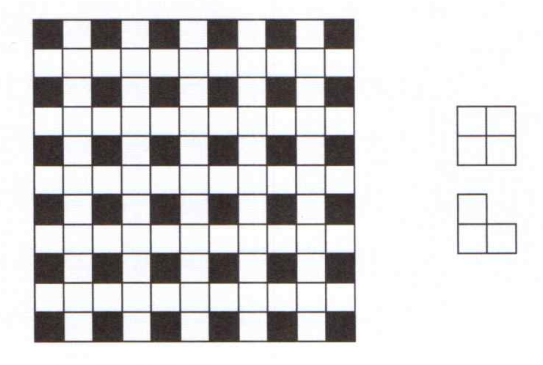
\includegraphics[width=1\linewidth]{imagens_8FMA121/imagem1}
	
	Sejam $x$ a quantidade de peças quadradas e $y$ a quantidade de peças em formato de $L$. \\
	a) Mostre que 4x + 3y = 121 \\\\
	b) Considerando as quantidades de casinhas pintadas que cada peça pode cobrir, mostre que são necessárias pelo menos 36 peças para cobrir o tabuleiro. \\\\
	c) Mostre que são necessárias pelo menos 23 peças em formato de $L$ para cobrir o tabuleiro. Nesse item, você \textbf{não} precisa apresentar um preenchimento do tabuleiro usando exatamente 23 peças em formato de $L$.	
	\newpage
	\begin{multicols}{2}
		\begin{enumerate}
			\setcounter{enumi}{2}
			\item O conjunto dos valores de $x$ reais que satisfazem o sistema de inequações $x^2 + 8x - 20 > 0$ e $x^2 + 5x < 0$ é:
			\begin{enumerate}[a)]
				\item $V = [-5; 0]$
				\item $V = \varnothing$
				\item $V = ]-10; -5[ \cup ]2; +\infty[$
				\item $V = ]-10; 2[$
				\item $V = \mathbb{R}$
			\end{enumerate}
			\item A solução do sistema \\ $\begin{cases} x + 2 \geq 3 \\ 3x^2 - 4x < x^2 + 7 \end{cases}$ \\ no universo dos reais é:
			\begin{enumerate}[a)]
				\item $V = ]-\infty; -1[ \cup \left]1 + \frac{3 \sqrt{2}}{2}\right[$
				\item $V = \mathbb{R} - \left\{ -1; 1 + \frac{3\sqrt{2}}{2}\right\}$
				\item $V = \varnothing$
				\item $V = \left[1; 1 + \frac{3\sqrt{2}}{2}\right]$
				\item $V = \mathbb{R}$
			\end{enumerate}
			\item Sendo $A = \{x \in \mathbb{R} | 5x - x^2 \leq 0\}, B = \{x \in \mathbb{R} | 4 < x \leq 5 \}$ e $C = \{x \in \mathbb{R} | x = 0\}$, então $X = (A \cap B) \cup C$ possui:
			\begin{enumerate}[a)]
				\item zero elementos.
				\item um único elemento.
				\item exatamente dois elementos.
				\item exatamente três elementos.
				\item infinitos elementos.
			\end{enumerate}
			\item A solução do sistema \\ 
			$
			\begin{array}{rcl|c}
			 \vline & x^2 + 5x - 2 < 0\\
			 \vline & \text{ou} \\
			 \vline & x^2 - 7x > 0 \\
			\end{array}
			$, \\ em $U = \mathbb{R}$, é:
			\begin{enumerate}[a)]
				\item $V = \left]-\infty; \frac{-5+\sqrt{33}}{2} \right[ \cup~]7;+\infty$
				\item $V = \left] \frac{-5 + \sqrt{33}}{2}; 7 \right[$
				\item $V = ]0; 7] \cup \left\{\frac{-5-\sqrt{33}}{2} \right\}$
				\item $V = [0; 1[ \cup [7; +\infty[$
				\item $V = \mathbb{R} - 7$\newpage
			\end{enumerate}
			\item Resolver os sistemas a seguir ($U = \mathbb{R}$):
			\begin{enumerate}[a)]
				\item $
				\begin{array}{rcl|c}
				 \vline & \frac{x^2 + 12x}{x^2 - 5x + 6} < 0 \\
				 \vline & \\
				 \vline & \frac{-x^2 + 4x + 7}{x - 9} \geq 0  \\
				\end{array}
				$
				\newpage
				\item $ 
				\begin{array}{rcl|c}
				 \vline & \frac{x^2 + 7x - 11}{3x^2 - 8x} \leq 0 \\
				 \vline & \\
				 \vline & \text{ou}\\
				 \vline & \\
				 \vline & \frac{x^2 + 12x + 11}{x^2 +24x - 25} \geq 0  \\
				\end{array}
				$\newpage
			\end{enumerate}
		\end{enumerate}
	\end{multicols}
	\begin{enumerate}
		\setcounter{enumi}{7}
		\item O conjunto solução do sistema $\begin{array}{rcl|c}
			\vline & 4x^2 + 6x < 0 \\
			\vline & \\
			\vline & \text{ou}\\
			\vline & \\
			\vline & x^2 -4 \geq 0 \\
		\end{array}
		$, em $U = \mathbb{R}$, é:
		\begin{enumerate}[a)]
			\item $\left\{ x \in \mathbb{R} | -2 < x < -\frac{3}{2}~\text{ou}~0 < x < 1~\text{ou}~x \geq 2 \right\}$
			\item $\{x \in \mathbb{R} | -2 < x < 0~\text{ou}~x \geq 2\}$
			\item $\{x \in \mathbb{R} | x = -1~\text{ou}~1 < x \leq 2~\text{ou}~x > 6\}$
			\item $\{x \in \mathbb{R} | x < -1~\text{ou}~0 \leq x \leq 2\}$
			\item $\left\{x \in \mathbb{R} | x \leq -2~\text{ou}~-\frac{3}{2} < x < 0~\text{ou}~x \geq 2 \right\}$ \newpage~
		\end{enumerate}
		\item O menor número que satisfaz o sistema $ 
		\begin{array}{rcl|c}
			\vline & 4x > 7 \\
			\vline & \\
			\vline & x^2 - 7x \geq -6 \\
		\end{array}
		$, em $U = \mathbb{R}$, é:
		\begin{enumerate}[a)]
			\item 1
			\item 2
			\item 5
			\item 6
			\item 10 \newpage
		\end{enumerate}
		\item Os valores de x reais que satisfazem o sistema $ 
		\begin{array}{rcl|c}
			\vline & 5x - 7 \leq 0\\
			\vline & \\
			\vline & \text{ou}\\
			\vline & \\
			\vline & x^2 - 4x + 3 > 0 \\
		\end{array}
		$ 
		\begin{enumerate}[a)]
			\item $1 < x \leq 3~\text{ou}~x > 7$
			\item $x < -2~\text{ou}~x > 3$. 
			\item $x \leq \frac{7}{5}~\text{ou}~x \geq 3$.
			\item $1 < x \leq 5$.
			\item $x \leq 1~\text{ou}~\frac{7}{5} < x < 3$.
		\end{enumerate}
	\end{enumerate}
\end{document}